\documentclass{article}
\usepackage[utf8]{inputenc}
\usepackage{amsmath}
\usepackage{graphicx} 
\usepackage[slovene]{babel}
\usepackage[a4paper,top=2cm,bottom=2cm,left=3cm,right=3cm,marginparwidth=1.75cm]{geometry}


\usepackage{amsmath}
\usepackage{graphicx}
\usepackage[colorlinks=true, allcolors=blue]{hyperref}

\title{Carving}
\author{Kunc Gregor, Jerič Vid}

\begin{document}
\maketitle

\section{Zgodovina Carvinga}

\subsection*{Razvoj tehnike}
Carving je tehnika ki je bila razvita na začetku 20. stoletja. Izumitelj te tehnike je bil Francoz "Georges Joubert", ki je uporabljal smuči s povečanim stranskim lokom.
Pri carvingu gre za tehniko pri kateri se zavija brez stranskega oddrsavanja smuči "Driftanja smuči".
Smučka je za tiste čase zelo nenavadna saj je na sprednjem delu zelo široka, na zadnjem pa zelo ozka.
Cilj pri karvingu je da se smučka med zavijem zareže v sneg po celi dolžini smučke. Smučarji so pri uporabi te tehnike zelo hitrejši, zavoji so pa daljši in bolj krožni. 
Pri tem morajo smučarji paziti da sta obe nogi med zavojem enako obremenjeni. 

DODAJ SLIKO

\subsection*{Razvoj materialov}
Carving smuči so skozi svoje obdobje doživele veliko sprememb v obliki in materialih.
Ta so smučarjem omogočale bodisi boljšo varnost, zmogljivost, udobje itd..
Ob zgodnjem času carvinga so bile smučke bolj ali manj izdelane predvsem iz lesa.
Te so bile težke, manj odzivne in težko so se prilagajale raznim razmeram okolice oz. smučišča.
S časoma so se pojavili tudi kompoziti s steklenimi vlaknami ter raznimi kovinami.
Te so smučkam izboljšale lasnosti kot so trdota in odzivnost.


Med 80-im desetletjem 19. stoletja so se na trgu začele pojavljati nove plastične carving smuči.
Te so od prejšnih ponujale več prilagodljivosti. Poleg tega so bile cenejše za izdelavo saj je bila plastika boljša za oblikovanje kot les.
Smuči so bile tudi marginalno lažje od predhodnih lesenih smuči.


Takoj po 80-tem deseletju 19 stoletja so se pojavile nove oblike carving smuči. Te so bile parabolične oblike. Tukaj se materiali niso kaj preveč spremenili
spremenila pa se je oblika smuči, kar je omogočalo boljše in lažje polaganje ovinkov.


Razvoj smuči se je potem kasneje bolj fokusiral na kombinacijo materialov.
Kombinacijski materiali ki v velikem deležu prisotnu še danes so: 
\begin{itemize}
    \item Karbonska vlakna
    \item Aluminij
    \item Titan
    \item Razni kompotizi lesa, plastike itd..
\end{itemize}
Te materiali so še izboljšali odzivnost smučk ter zmanjšale izgubo hitrosti pri smučarjih.

\*

Poleg tega da imamo razne materiale iz katerih so carving smučke izdelane, je pomembna tudi obdelava smuči.
Ta obdelava vključuje razne obloge in premaze. Te so smučkam postale pomembne saj so izboljšale drsenje ter zmanjšale trenje. 
Ta so se skozi leta tudi razvila in omogočila boljše lasnosti.

DODAJ SLIKO

\subsection*{Tehnologija}
Razvoj tehnologije pri carving smučeh se je skozi leta razvijal paralelno z izborom materialov.
Neke ključne tehnološke inovacije skozi leta so:
\begin{itemize}
    \item Parabolična oblika smuči
    \item Napredna konstrukcija
    \item Sodobni "inteligentni" materiali
    \item Amortizacija in blaženje
    \item Razvoj profilov smuči
    \item Uporaba računalniškega modeliranja
\end{itemize}

\*

Razvoj tehnologije smuči skozi leta je zaznamovan z inovacijami v materialih, oblikovanju smuči, konstrukciji smuči, kar omogoča smučarjem izkušnjo, ki je bolj prilagojena njihovim željam in sposobnostim.

DODAJ SLIKO

\subsection*{Infrastruktura}
Z vzponom in razvojem karvinga je teno povezana tudi infrastruktura ki jo spremlja.
Carving smuči zajema zelo različna področja infrastrukture. Zajema vse od smučarskih prog in centrov, območij za testiranje fizikalnih lasnosti smuči, trgovin ter samih tovarn kjer same smuči izdelajo.

Smučarski centri in proge so zelo tesno povezane saj so ključna destinacija, kjer smučarji izvajajo tehniko carvinga.
Razvite so bile posebne proge katere so prilagojene za carving. Te proge vključujejo primerno oblikovanje zavojev izključno za carving.
Smučarski centri so pogosto v ospredju, ko gre za preizkušanje in izboljševanje smuči.

Laboratoriji oz. inovacijski centri so pomembni saj se proizvajalci smuči pogosto zanašajo na sam razvoj smuči.
Zelijo imeti čim cenejši ter boljši izdelek na trgu. Ti centri so ključen del izboljšav karvinga skozi njegovo življensko obdobje.

Trgovine so pomemben del povezane infrastrukture, saj smučarjem omogočijo dostop do najnovejše in najnaprednejše opreme, vključno s carving smučmi. 
Poleg tega osebje v trgovinah lahko pomagajo pri izbiri karving smuči, katere bi bile najbolje primerne za kupca.

Poleg tega je pomemben del infrastrukture tudi virtualna infrastruktura kot so na primer oglasi ali spretne informacije oz. spletni članki testov smuči.
Ta ponuja novemu kupcu opcijo da si lahko sam izbere smuči po njegovih potrebah oz. finančnih zmožnostih.

\subsection*{Tehnologija smuči pri tekmovalcih ter rekreativcih}
Tehnološa razlika med obema je predvsem izražena v stopnji specializacije ter zahtevnosti pri posamični skupini.
Tekmovalci in rekreativci imajo različne prioritete pri izbiri smuči.

Ena izmed njih je uporabljen material pri izdelavi. Smučke za rekreativce so narejene večinoma iz bolj cenovno dostopnih materialov. 
V primerjavi s smučmi ki jih ima tekmovalec so manj naprednejše. To načeloma ni slabo saj so bolj odpuščajoče za napake, ter so bolj prilagojene sproščenemu smučanju.
Tekmovalne so pa izdelano iz kompozitov materialov, ki omogočajo izjemno trdoto, nizko težo in hitro odzivnost. 

Ena ključnih razlik je tudi oblika. Tekmovalci imajo pogosto bolj agresiven profil, ki jim omogoča boljši oprijem in stabilnost pri veliki hitrosti.
Pri tekmovalcihg to vključuje kombinacijo "rockerja" in "camber" profila, ki sta prilagojena glede na disciplino (slalom, veleslalom, smuk...).
Medtem ko pri rekreativcih so profili usmerjeni bolj na zmerno stran. Ta jim omogoča enostavnejše upravljanje in manevriranje. 
Te so namenjene udobju in zabavi.

Poleg same oblike je pomembna tudi velikost in lasnost geometrije. Ta je pri tekmovalcih zelo specifična, glede na njihov slog in disciplino.
Velikokrat imajo tekmovalci krajše in bolj obrnjene smuči za boljšo okretnost.
Pri rekreativcih je velikost in oblika zelo variabilna in odvisna od želje uporabnika (lažje učenje, bolj mehko smučanje...).

Seveda je glavni faktor pri tehnologiji tudi cena izdelave oz. razvoja. Tekmovalci imajo na voljo ponavadi veliko več finančne podpore kot nekdo, ki se s smučanjem ukvarja rekreativno.
Zaradi te cenovne razlike imajo tekmovalci tudi najnovejše in najbolje tehnološko razvite materiale.
\subsection*{Razvoj varosti pri smučeh}
DODAJ TA DEL

DODAJ SLIKO
\pagebreak

\section{Fizika pri smučarski tehniki carving}

Carving smučanje je zelo zanimivo in zabavno. Iz vidika smučarja in iz vidika fizike, ki se pojavi.
Pri carvingu se smučarji trudijo izvajati zavoje z visoko nagibnim kotom in majhnim radijem (seveda odvisno od hitrsoti in smuči, ki jih ima). 
Glavni fizikalni koncepti, ki vplivajo na carving, vključujejo zakone kinematike pri kroženju in drugi zakoni, ki jih bomo spoznali. \\ \newline
Pri carvingu se smučar nagne v zavoj in uporablja robove smuči, da ustvari ovinek. Ključna sila, 
ki omogoča carving, je sila stranice smuči. Ko se smučar nagne v zavoj, se težišče premakne, kar ustvarja nagnjenost silnice. 
To povzroči, da se smučka začne obračati okoli svoje osi, kar omogoča elegantno izvajanje zavojev (seveda je odvisna od oblike in radijem ki ga smučka dopušča).\\ \newline
Pomembno vlogo igra tudi trenje med smučko in snegom. Visokokakovostne carving smuči imajo posebne oblike in strukture, 
ki izboljšujejo stik s snegom in zmanjšujejo trenje, kar omogoča boljši nadzor in večjo stabilnost med carvingom.

\subsubsection*{Razlike med carving tehniko in staro tehniko oddrsavanja}

V resnici je glavna razlika v trenju. Pri oddrsavanju prihaja do stalnega visokega trenja ob snežno podlago, ki omogoča da smučar zavije.
Pri carvingu pa temu ni tako! Carving tehnika pa omogoča smučarju da izpoelje zavoj in pri njem celo pridobiva hitrost, saj je trenje tako majhno. 
V naslednjih poglavjih predstavimo zakaj.

\subsection*{Sile pri carving smučanju}
Predpostavimo da na smučarja ne deluje zračni upor. \\ \newline
Tako opazimo da ko je smučar na ravno podlagi in se ne giba deluje sila zemlje na smučarja ter podaga z enako normalno silo na smučarja. 
Ko se smučar postavi na klančino in ne zavija in se pelje naravnost na njega deluje sila podlage na smučarja pravokotno kot smuči (če je podlaga ravna),
ter sila zemlje na smučarja deluje pod kotom kot je strma strmina po kateri se pelje. Pri gibanju nastane tudi sila trenja, ki je odvisna od 
sile normale na smuči ter stika s podlago ter materijalov. Zato se pri razlagi ne bomo spuščali v silo trenja tako da jo bomo v naprej zanemarili.
\begin{align}
    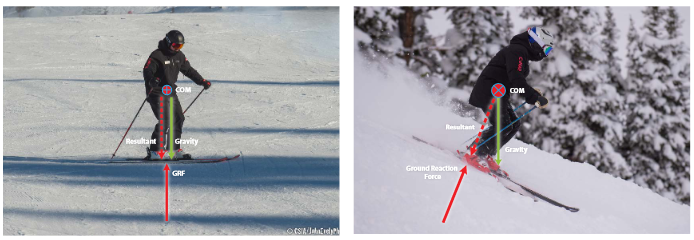
\includegraphics[scale=0.8]{../images/Screenshot 2023-12-03 152058.png}
\end{align}
\subsubsection*{Kako pa s silami ko se smučar nangne v zavoj}
Da bomo razumeli kaj se dogaja takrat moramo vedeti kakšne sile nastajajo pri vrtenju. Obravnavali bomo centripetelno in centrifugalno silo. \\ \newline
Ko se smučar nagne v zavoj mora svoje telo nagniti da klobuje razultanti sil, ki nastane pri zavoju na njegove smuči. \\ \newline
\textbf{To zgleda takole:} \newline 
Smučar se nagne in z pritiskom noge ustvari silo katero smuč "zapiči" v snešno podlago in smučko upogne. Na smučarja začne delovati nasptrotna sila zato mora ohranjati svoj naklon in tako pride do zavoja.
\begin{itemize}
    \item[1] Smučar s tem da se nagne ustvari centrifugalno silo, ki nastane saj začne zavijati.
    \item[2] Smučar se pri tem mora nagniti saj sila zemlje tudi deluje tako da je rezultanta sil 0. 
    \item[3] Tako rezultanta sil kaše natanko na mesto stika notranjega roba zunanje smučke v zavoju ter tako tudi nasprotno sila podlage na smuči pod istim kotom.
\end{itemize} 
Kot ki ga omenjamo je odvisen od radija in hitrosti, ki jo smučar ima. Saj sta te dve vresnosti odvisni od centrifulne sile, ki nastane pri zavoju. \\ \newline
Kot in velikost sile, ki deluje na podlago je odvisen tudi v katerem delu zavoja je smučar. Saj s tem ko opravi zavoj pritisk na smuči zmanjša in svoj nagib ter s tem zaključi zavoj.
\begin{align}
    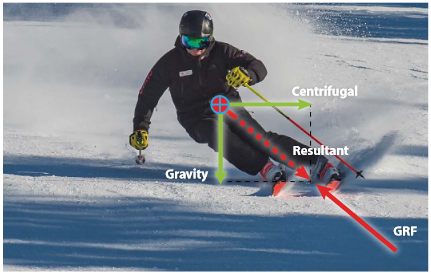
\includegraphics[scale=0.8]{../images/Screenshot 2023-12-03 152028.png}
\end{align}
\subsection{Bolj podrobno razumevanje fizike}
\textbf{Uprašajmo se zakaj smučarji uporabljajo palice za smučanje.} Odgovor najdemo v navoru na težišče smučarja.
Palice pomagajo, da je vsota navorov okoli težišča enaka 0. Kljub temu da so palice in roke veliko lažje kot
od teže smučarja prispevajo velik ravnotežni navor. \\ \newline
VSTAVI SLIKO
\textbf{Kaj pa razultanta sil če upoštevamo trenje.} Takrat pa se nam spremeni smer sile podlage na smučarja.
Silo podlage si lahko predstavljamo da je sestavljena iz komponent sile normale in sile trenja. 
Tako se tudi težišče smučarja premakne "nazaj" oz. če gledamo težišče kot točko se ta točka nahaja na vektorju
sile podlage na smučarja. \\ \newline

VSTAVI SLIKO KJER JE SMUČAR NANGNJEN ZARADI TRENJA
\subsubsection*{Stara tehnika}
Pri stari tehniki, ki smo jo že omenili prej pride do zavijanja zaradi razliki v navorih. Saj iz slike sledeče vidimo
da je repni del smuči krajši od sprednjega dela se smučka zasuka. Oz je večja površina izpostavljena trenju s snežno površino.
\subsubsection*{Nova carving tehnika}
Kot smo prej omenili je pri te tehniki pri smučarju še bolj pomembno, da ohranja ravnotežni položaj. Da smučar lahko zavije mora na njega delovati
centrifugalna sila oz radialna sila ki jo zapišemo kot.
\[F_c=\frac{mv^2}{r}\]
Izpeljava iz $ F_c=ma_r $ \\ \newline
Kjer je r polmer krožnice, v je tangenta hitrost, smer sile $ F_c $ pa kaže proti središču kroženja. Centripetalna sila je sorazmerna z kvadratom hitrosti
zato se mora smučar ustrezno nagniti, da ohranja prečni ravnotežni položaj (ohranni vsoto vseh sil in navorov okoli težišča 0).
Če si predstavljamo nato silnice na smučarja mora smučar ob večji hitrosti se veliko bolj nagniti da ohrani ravnovesje sil kot pa pri majhni hitrosti 
če želi izpeljati enak ovinek kot pri nizki hitrosti.\\ \newline 
\begin{align}
    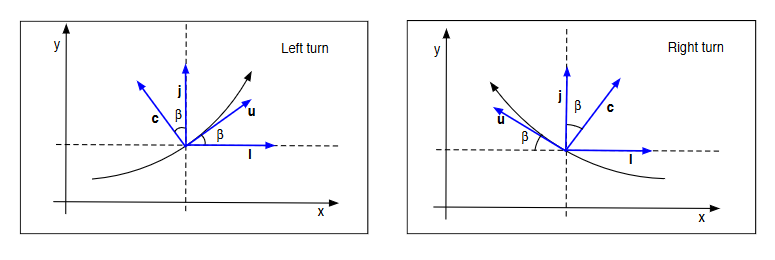
\includegraphics[scale=0.6]{../images/Screenshot 2023-12-03 151902.png} \\
    \text{TE DVE SLIKI BI JAZ NANOVO NARISAL IN DAL PRAVE OZNAKE}
\end{align}

\textbf{Vendar kako smučar pridobi hitrost}
Ta pojav lahko opišemo z energijami. Upoštevamo da deluje na smuči stalen pojem oz. sila trenja, ki ga opišemo kot delo $ A $. Zračni upor pa zanemarimo.\newline
Opazujemo položaj 1 ko je smučar na vrhu hriba ter položaj 2 ko je smučar na dnu hriba. In za sistem gledamo smučarja in zemljo.

\[Wp_1+A_t=Wk_2\]
Tako lahko izvemo kolikšno hitrost lahko razvije z našimi predpostavkami. 
\[Wk=\frac{mv^2}{2}\]
Moramo vedeti da pri carving smučanju smučar pridobiva (do neke mere) hitrostu tudi pri samem zavinaju, saj trenje ni tako veliko v smeri gibanja.
S pravilno tehniko lahko smučar stalno pridobiva hitrost saj je stik s snežno površino zelo majhen. Če predpostavimo prfektne pogoje ter 
sneg z lastnosti da nam to omogoča bi v teoriji lahko smučar pridobil ogromne hitrosti. (seveda moramo predpostaviti tudi da smučarjevo telo take sile lahko prenese)
\section{Zakluček}
Če strnemo misli lahko vidimi da lahko pri opazovalnem sistemu smučarja govorimo o ogromno fizikalnih pojavov. Kot primer energije, bi 
lahko obravnavali energije ki nastanejo pri zavijanju itd. Zato smo v tem seminarju opisali samo osnovne pojave.

DOKONČAJ
\end{document}